\section{实验结果}

\subsection{静态法测 \ce{CCl4} 的饱和蒸气压}

\subsubsection{常压下 \ce{CCl4} 的沸点}

充分排气后,测量常压下 \ce{CCl4} 的沸点,如表 \ref{tab:1} 所示。

\begin{table}[htbp]
    \centering
    
    \bicaption{常压下 \ce{CCl4} 的沸点}{Boiling Point of Carbon Tetrachloride at Atmospheric Pressure}
    \begin{tabular}{cc}
    \toprule
    \( p \) /\si{kPa} & \( T \) /\si{\celsius} \\
    \midrule
    99.95 & 75.79 \\
    99.94 & 75.83 \\
    99.93 & 75.83 \\
    99.93 & 75.82 \\
    \bottomrule
    \end{tabular}
    \label{tab:1}
\end{table}

根据表 \ref{tab:1},使用 numpy 求得 \ce{CCl4} 常压下的沸点为 \( 75.82 \)\si{\celsius},沸点的标准差为 \( 0.02 \)\si{\celsius},最终,换算为热力学温标,\ce{CCl4} 常压下的沸点为
\[
T_b = 348.97 \pm 0.02 \si{\celsius}
\]

\subsubsection{不同气压下 \ce{CCl4} 的饱和蒸气压}

使用静态法测定不同压力下 \ce{CCl4} 的沸点 \(t_b\),将气压取对数 \(\ln \dfrac{p}{p^\ominus}\)、温度转化为热力学温标后取倒数 \(T^{-1}\times10^{3}\),结果如表 \ref{tab:2}、图 \ref{fig:1} 所示。标准大气压取 \(p^\ominus=100.00\si{~kPa}\),摄氏温度通过 \(T = t + 273.15\si{~K}\) 转化为热力学温度。

\begin{table}[htbp]
    \centering
    \bicaption{\ce{CCl4} 饱和蒸气压$p$-温度$T$的测定与数据处理}{Measurement and Data Analysis of the SVP $p$ vs. Temperature $T$ for \ce{CCl4}}
    \begin{tabular}{ccccc}
        \toprule
        $p$/\si{kPa} & $\ln\dfrac{p}{p^\ominus}$ & $t$/\si{\celsius} & $T$/\si{K} & $T^{-1}\times10^{3} $/$\mathrm{K^{-1}}$ \\
        \midrule
        99.93 & -0.0007002 & 75.82 & 348.97 & 2.8656 \\
        95.30 & -0.04814 & 74.23 & 347.38 & 2.8787 \\
        89.95 & -0.1059 & 72.38 & 345.53 & 2.8941 \\
        84.97 & -0.1629 & 70.64 & 343.79 & 2.9088 \\
        79.59 & -0.2283 & 68.63 & 341.78 & 2.9259 \\
        74.96 & -0.2882 & 66.83 & 339.98 & 2.9413 \\
        67.22 & -0.3972 & 63.67 & 336.82 & 2.9689 \\
        64.15 & -0.4439 & 62.32 & 335.47 & 2.9809 \\
        59.57 & -0.5180 & 60.18 & 333.33 & 3.0000 \\
        57.04 & -0.5614 & 58.98 & 332.13 & 3.0109 \\
        53.73 & -0.6212 & 57.29 & 330.44 & 3.0263 \\
        50.23 & -0.6886 & 55.42 & 328.57 & 3.0435 \\
        \bottomrule
    \end{tabular}
    \label{tab:2}
\end{table}

\begin{figure}[htbp]
    \centering
    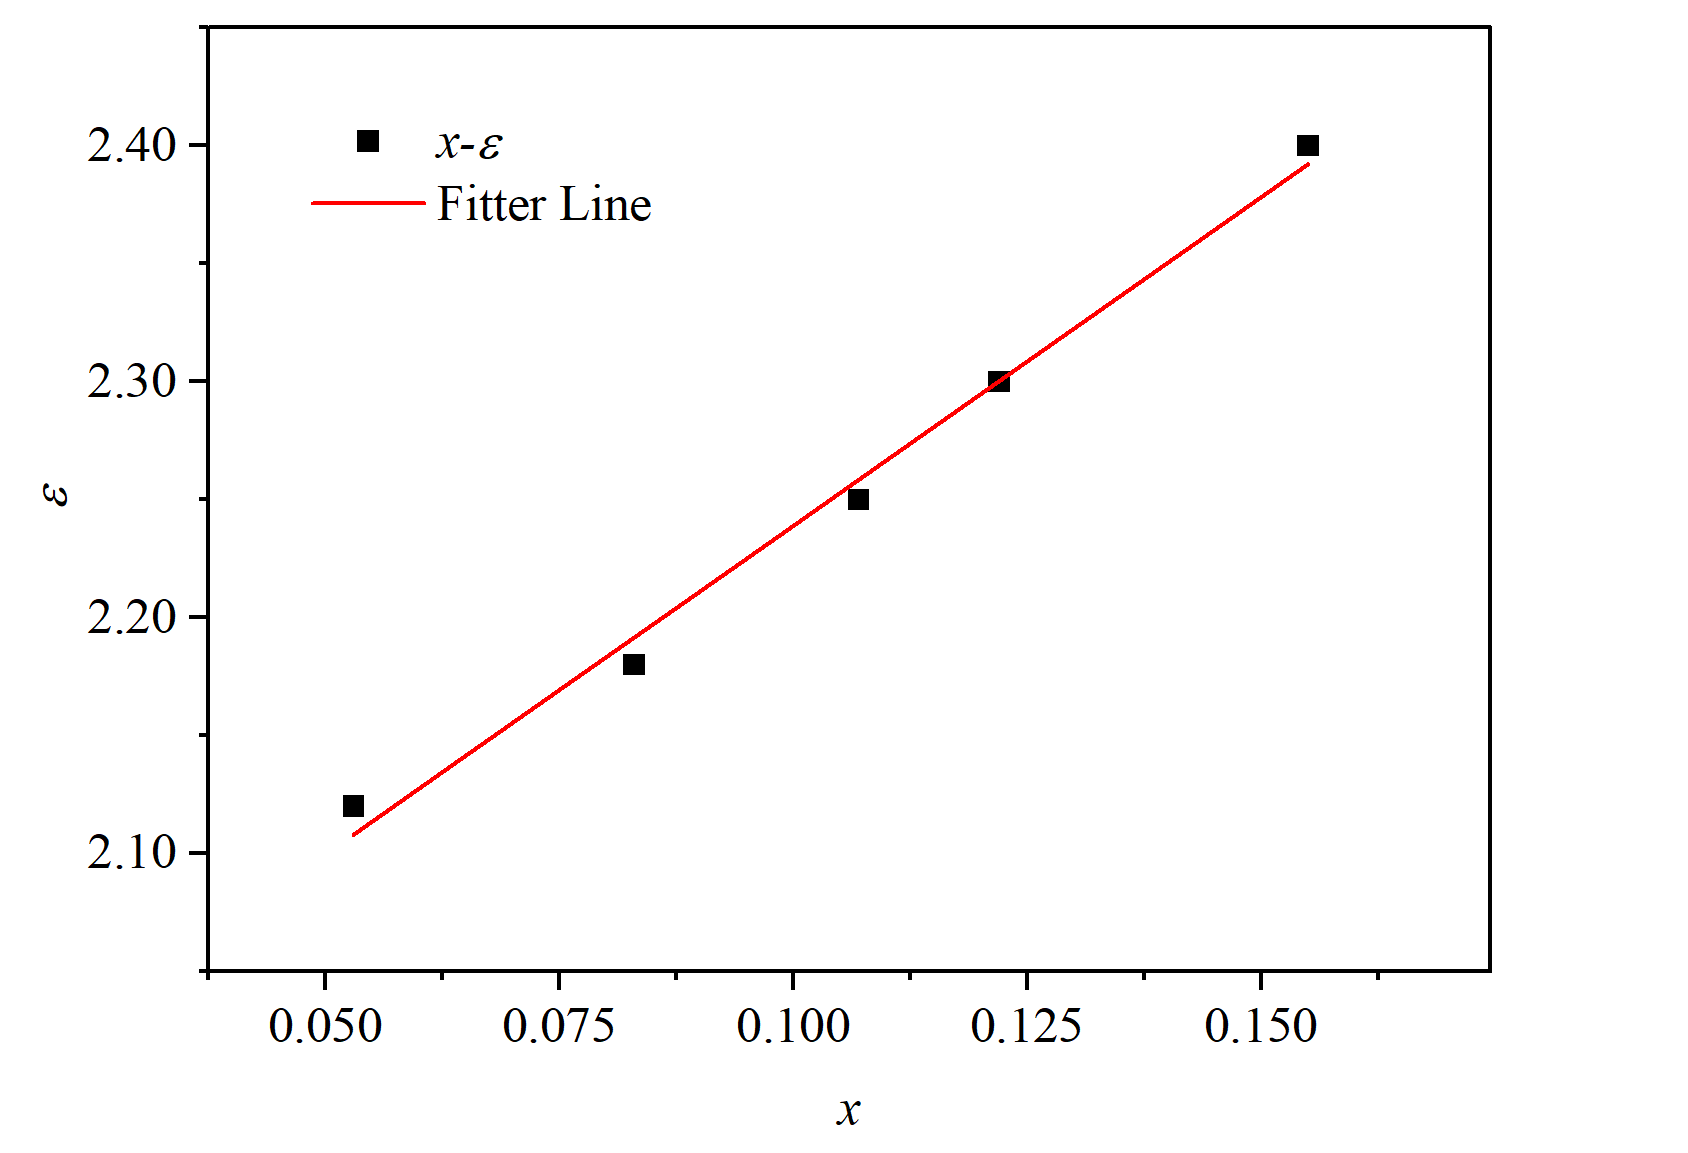
\includegraphics[width=.78\textwidth]{figures/1-1.png}
    \bicaption{\ce{CCl4} 饱和蒸气压$p$-温度$T$的测定曲线}{Determination Curve of SVP $p$ vs. Temperature $T$ for \ce{CCl4}}
    \label{fig:1}
\end{figure}

根据 Clausius-Clapeyron 方程,饱和蒸气压 $p$ 与气液平衡温度 $T$ 之间满足
\begin{equation}\label{eq:1}
    \lg \frac{p}{p^{\ominus}}=-\frac{\Delta_1^{g} H_m}{RT}+\frac{\Delta_1^{g} S_m}{R}
\end{equation}

\begin{figure}
    \centering
    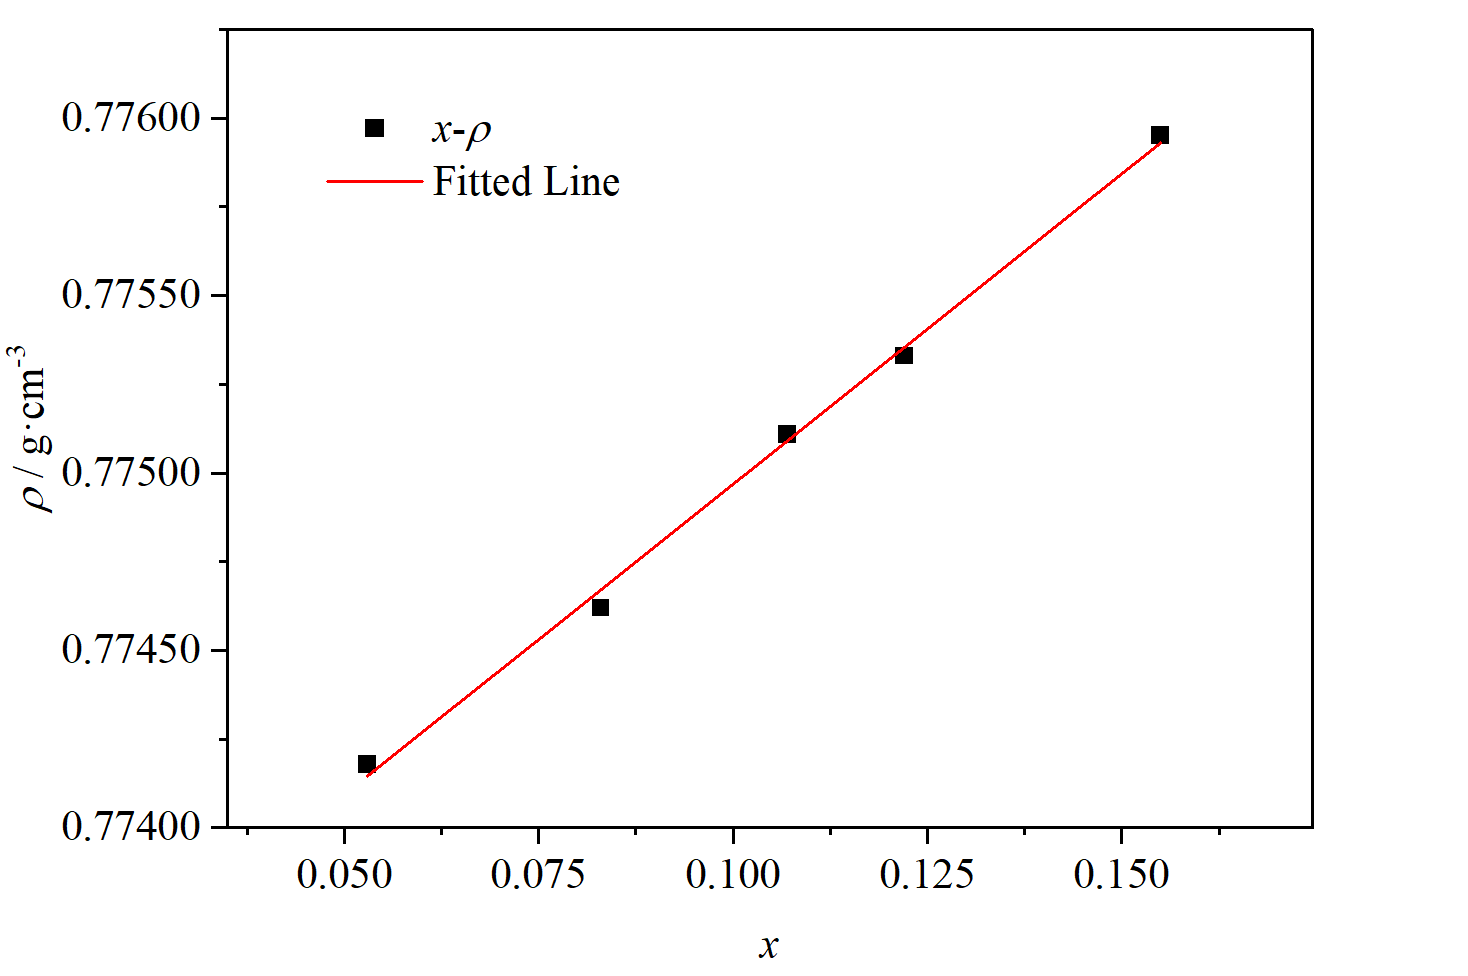
\includegraphics[width=.78\textwidth]{figures/1-2.png}
    \bicaption{{\ce{CCl4} 的\(\ln \dfrac{p}{p^\ominus}-T^{-1}\times10^{3}\) 拟合直线}}{Fitting Line of \(\ln \dfrac{p}{p^\ominus}-T^{-1}\times10^{3}\) for \ce{CCl4}}
    \label{fig:2}
\end{figure}

根据表 \ref{tab:2} 中的数据,使用\texttt{scipy.stats.lingress} 与 \texttt{scipy.optimize.cruve\_fit} 对 \(\ln \dfrac{p}{p^\ominus}\) 与 \(T^{-1}\times10^{3}\) 进行 $y=ax+b$ 的线性拟合并求出拟合误差,对 \(\ln \dfrac{p}{p^\ominus}\) 与 \(T^{-1}\times10^{3}\) 作图,得到图 \ref{fig:2}。

拟合直线的表达式为:
\[
    \ln \dfrac{p}{p^\ominus} = (-3.882 \pm 0.009)\dfrac{T^{-1}\times10^{3}}{\mathrm{K^{-1}}} + (11.13\pm 0.03);\quad R^2 = 0.99994
\]

\subsubsection{\ce{CCl4} 相关物理量的计算}

根据直线拟合公式外推,可以求出 \ce{CCl4} 在实际大气压 \SI{101.325}{kPa} 下的沸点:
\[
T_{101.3 \mathrm{kPa}}=\frac{a}{\ln \frac{b}{p^{\otimes}}-b}=349.3 \mathrm{~K}
\]
计算温度的不确定度:
\[
\sigma_T=T \sqrt{\left(\frac{\sigma_a}{a}\right)^2+\left(\frac{\sigma_b}{\ln \frac{p}{p^{\ominus}}-b}\right)^2}=1.2 \mathrm{~K}
\]
最终得到 \ce{CCl4} 在实际大气压 \SI{101.325}{kPa} 下的沸点为:
\[
T = (349.3\pm1.2) \mathrm{~K} = (76.1\pm1.2)\si{\celsius}
\]

查阅 \textit{CRC Handbook of Chemistry and Physics}\cite{haynes2016crc},可知 \ce{CCl4} 在 \SI{101.325}{kPa} 下的沸点 $T = 76.7\si{\celsius}$,实验结果与文献值仅差$-0.8\%$,非常接近。

进一步地,根据\eqref{eq:1},可以得到:
\[
\begin{aligned}
    \Delta_1^{g} H_m &= R\times a\times 10^{3} = (3.228\pm0.008)\times10^{4}\mathrm{~J\cdot mol^{-1}} = (32.28\pm 0.08)\mathrm{~kJ\cdot mol^{-1}}\\
    \Delta_1^{g} S_m &= R\times b = (92.53\pm 0.23)\mathrm{~J\cdot mol^{-1}\cdot K^{-1}}
\end{aligned}
\]

查阅 \textit{CRC Handbook of Chemistry and Physics}\cite{haynes2016crc},可知 \ce{CCl4} 在标准大气压的沸点下的 $\Delta_1^{g} H_m$ 为 $29.82\mathrm{~kJ\cdot mol^{-1}}$,实验值与文献值相差$+8\%$,偏差略大。

根据褚鲁统规则,在常压沸点下各正常液体的摩尔熵近似相同,约为 $88 \mathrm{~J} \cdot \mathrm{K}^{-1} \cdot \mathrm{mol}^{-1}$ 。实验得到 \ce{CCl4} 摩尔气化熵的计算结果与禇鲁统规则相差$+5\%$,比较接近。


\subsection{动态法测 \ce{H2O} 的饱和蒸气压}

\subsubsection{不同气压下 \ce{H2O} 的饱和蒸气压}

该部分根据同学的提问:
\begin{enumerate}
    \item 在不同的气压下,当温度达到沸点时,会有一段的平台区,但是该平台区的温度并非保持不变的,而是会逐渐升高,取平台区不同阶段的温度会对结果造成怎样的影响?
    \item 当气压达到环境大气压后,测定水的沸点温度是否会随着时间的变化而发生变化?
\end{enumerate}

针对这两个问题,在使用静态法测定不同压力下 \ce{H2O} 的沸点 \(t_b\)时,分别取三个温度-气压:
\begin{enumerate}
    \item $p_1,T_1$为刚达到平台区时的温度与气压;
    \item $p_2,T_2$为平台区快结束前的温度与气压;
    \item $p,T$为$p_1,T_1$、$p_2,T_2$的平均温度与平均气压。
\end{enumerate}
将气压取对数 \(\ln \dfrac{p}{p^\ominus}\)、温度转化为热力学温标后取倒数 \(T^{-1}\times10^{3}\),结果如表 \ref{tab:3}、表 \ref{tab:4}、表 \ref{tab:5}、图 \ref{fig:3} 所示。标准大气压取 \(p^\ominus=100.00\si{~kPa}\),摄氏温度通过 \(T = t + 273.15\si{~K}\) 转化为热力学温度。

\begin{table}[htbp]
    \centering
    \bicaption{\ce{H2O} 饱和蒸气压$p_1$-温度$T_1$的测定与数据处理}{Measurement and Data Analysis of the SVP $p$ vs. Temperature $T$ for \ce{H2O}}
    \begin{tabular}{ccccc}
        \toprule
        $p_1$/\si{kPa} & $\ln\dfrac{p_1}{p^\ominus}$ & $t_1$/\si{\celsius} & $T_1$/\si{K} & $T_1^{-1}\times10^{3} $/$\mathrm{K^{-1}}$ \\
        \midrule
        51.57 & -0.6622 & 81.07 & 354.22 & 2.8231 \\
        54.89 & -0.5998 & 83.07 & 356.22 & 2.8072 \\
        59.29 & -0.5227 & 85.00 & 358.15 & 2.7921 \\
        64.94 & -0.4317 & 87.33 & 360.48 & 2.7740 \\
        69.53 & -0.3634 & 89.26 & 362.41 & 2.7593 \\
        74.65 & -0.2924 & 91.30 & 364.45 & 2.7438 \\
        79.77 & -0.2260 & 93.06 & 366.21 & 2.7306 \\
        84.69 & -0.1662 & 94.82 & 367.97 & 2.7176 \\
        89.70 & -0.10870 & 96.42 & 369.57 & 2.7058 \\
        94.79 & -0.05351 & 98.00 & 371.15 & 2.6943 \\
        99.84 & -0.001601 & 99.41 & 372.56 & 2.6841 \\
        \bottomrule
        \end{tabular}
    \label{tab:3}
\end{table}

\begin{table}[htbp]
    \centering
    \bicaption{\ce{H2O} 饱和蒸气压$p_2$-温度$T_2$的测定与数据处理}{Measurement and Data Analysis of the SVP $p$ vs. Temperature $T$ for \ce{H2O}}
    \begin{tabular}{ccccc}
        \toprule
        $p_2$/\si{kPa} & $\ln\dfrac{p_2}{p^\ominus}$ & $t_2$/\si{\celsius} & $T_2$/\si{K} & $T_2^{-1}\times10^{3} $/$\mathrm{K^{-1}}$ \\
        \midrule
        51.61 & -0.6615 & 81.30 & 354.45 & 2.8213 \\
        54.90 & -0.5997 & 83.18 & 356.33 & 2.8064 \\
        59.28 & -0.5229 & 85.44 & 358.59 & 2.7887 \\
        64.94 & -0.4317 & 87.53 & 360.68 & 2.7725 \\
        69.53 & -0.3634 & 89.47 & 362.62 & 2.7577 \\
        74.64 & -0.2925 & 91.26 & 364.41 & 2.7442 \\
        79.76 & -0.2261 & 93.07 & 366.22 & 2.7306 \\
        84.69 & -0.1662 & 94.89 & 368.04 & 2.7171 \\
        89.68 & -0.10892 & 96.41 & 369.56 & 2.7059 \\
        94.77 & -0.05372 & 98.00 & 371.15 & 2.6943 \\
        99.84 & -0.001601 & 99.34 & 372.49 & 2.6846 \\
        \bottomrule
        \end{tabular}
    \label{tab:4}
\end{table}

\begin{table}[htbp]
    \centering
    \bicaption{\ce{H2O} 饱和蒸气压$p$-温度$T$的测定与数据处理}{Measurement and Data Analysis of the SVP $p$ vs. Temperature $T$ for \ce{H2O}}
    \begin{tabular}{ccccc}
        \toprule
        $p$/\si{kPa} & $\ln\dfrac{p}{p^\ominus}$ & $t$/\si{\celsius} & $T$/\si{K} & $T^{-1}\times10^{3} $/$\mathrm{K^{-1}}$ \\
        \midrule
        51.59 & -0.6618 & 81.185 & 354.335 & 2.8222 \\
        54.90 & -0.5997 & 83.125 & 356.275 & 2.8068 \\
        59.28 & -0.5228 & 85.22 & 358.37 & 2.7904 \\
        64.94 & -0.4317 & 87.43 & 360.58 & 2.7733 \\
        69.53 & -0.3634 & 89.365 & 362.515 & 2.7585 \\
        74.64 & -0.2924 & 91.28 & 364.43 & 2.7440 \\
        79.76 & -0.2261 & 93.065 & 366.215 & 2.7306 \\
        84.69 & -0.1662 & 94.855 & 368.005 & 2.7174 \\
        89.69 & -0.1088 & 96.415 & 369.565 & 2.7059 \\
        94.78 & -0.05361 & 98.00 & 371.15 & 2.6943 \\
        99.84 & -0.001601 & 99.375 & 372.525 & 2.6844 \\
        \bottomrule
        \end{tabular}
    \label{tab:5}
\end{table}

\begin{figure}[htbp]
    \centering
    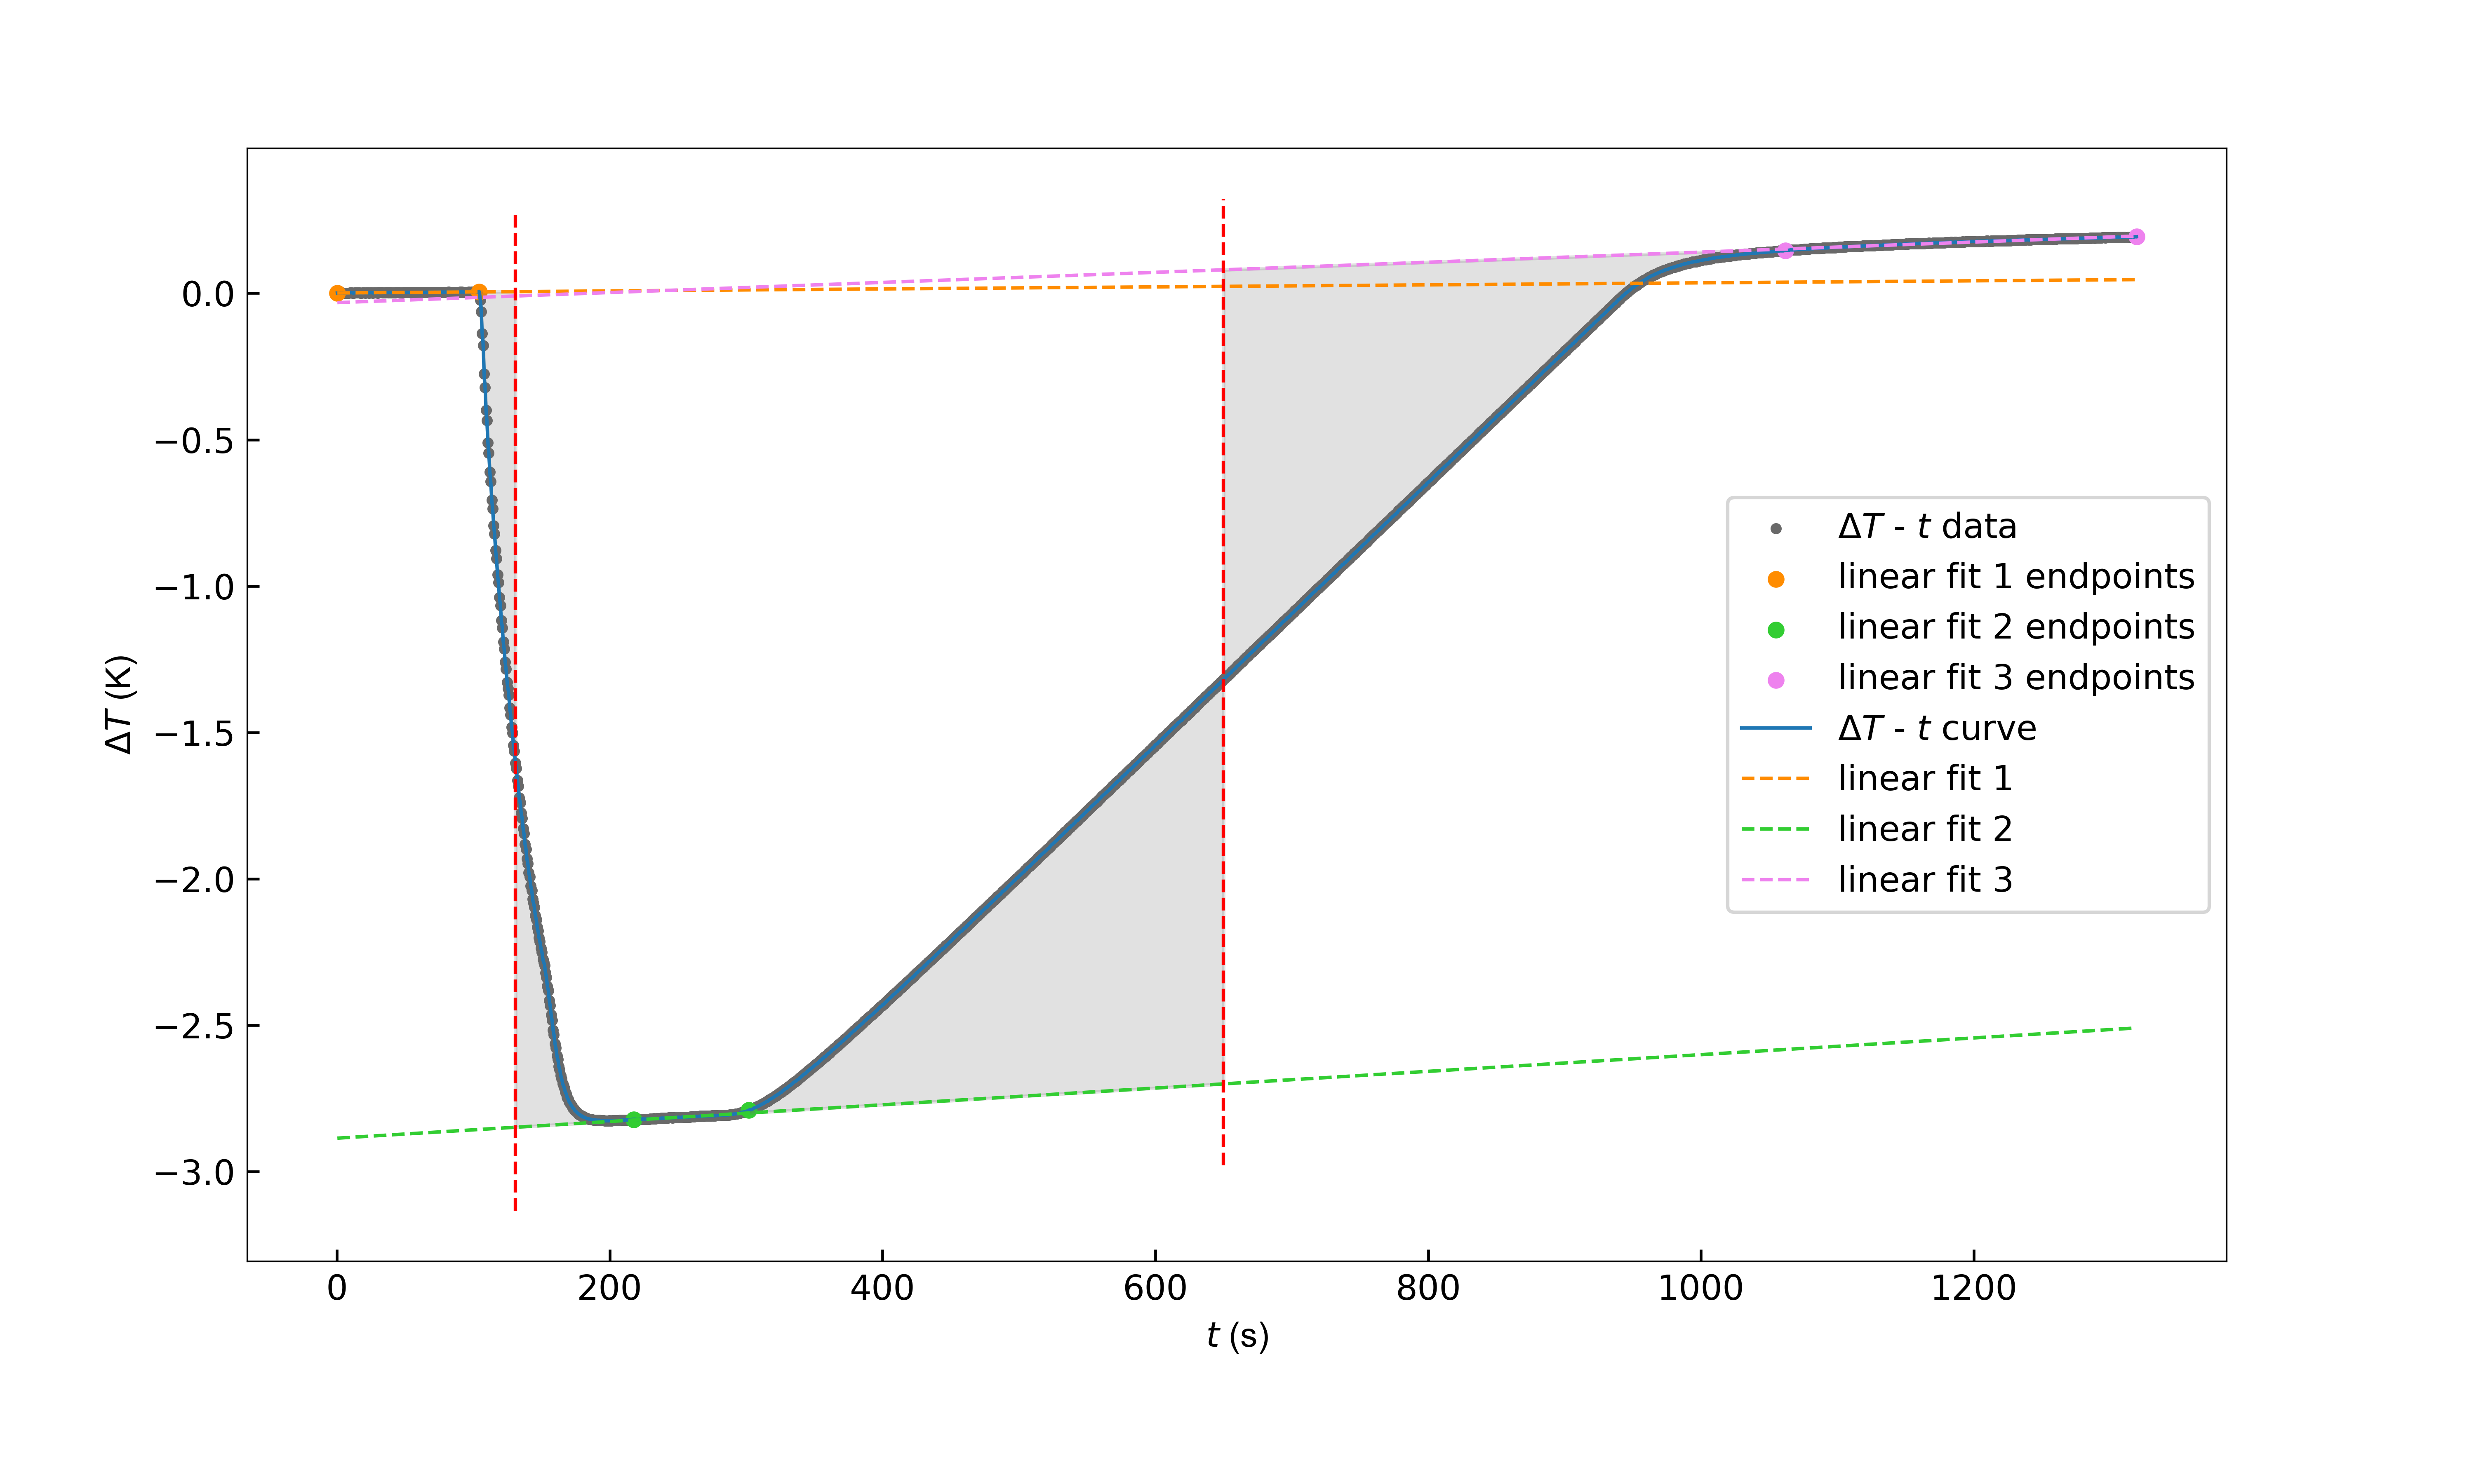
\includegraphics[width=.78\textwidth]{figures/2-1.png}
    \bicaption{三组\ce{H2O} 饱和蒸气压$p$-温度$T$的测定曲线}{Determination Curves of Saturated Vapor Pressure $p$ vs. Temperature $T$ for Three Sets of \ce{H2O}}
    \label{fig:3}
\end{figure}

根据表 \ref{tab:3}、表 \ref{tab:4}、表 \ref{tab:5} 中的数据,使用\texttt{scipy.stats.lingress} 与 \texttt{scipy.optimize.cruve\_fit} 分别对三组 \(\ln \dfrac{p}{p^\ominus}\) 与 \(T^{-1}\times10^{3}\) 进行 $y=ax+b$ 的线性拟合并求出各自的拟合误差,对三组的 \(\ln \dfrac{p}{p^\ominus}\) 与 \(T^{-1}\times10^{3}\) 作图,得到图 \ref{fig:4}。

\begin{figure}[htbp]
    \centering
    \includegraphics[width=.78\textwidth]{figures/2-2.png}
    \bicaption{三组 \ce{H2O} 的\(\ln \dfrac{p}{p^\ominus}-T^{-1}\times10^{3}\) 拟合直线}{Fitting Lines of \(\ln \dfrac{p}{p^\ominus}-T^{-1}\times10^{3}\) for Three Sets of \ce{H2O}}
    \label{fig:4}
\end{figure}

三组数据拟合直线的表达式分别为:
\begin{align*}
\ln \frac{p_1}{p^\ominus} &= (-4.78 \pm 0.03)\frac{T_1^{-1}\times10^{3}}{\mathrm{K^{-1}}} + (12.83 \pm 0.07); & R^2 &= 0.99976 \\
\ln \frac{p_2}{p^\ominus} &= (-4.87 \pm 0.04)\frac{T_2^{-1}\times10^{3}}{\mathrm{K^{-1}}} + (13.07 \pm 0.10); & R^2 &= 0.99950 \\
\ln \frac{p}{p^\ominus} &= (-4.82 \pm 0.03)\frac{T^{-1}\times10^{3}}{\mathrm{K^{-1}}} + (12.95 \pm 0.08); & R^2 &= 0.99971
\end{align*}

\subsubsection{\ce{H2O} 相关物理量的计算}

根据不同读数方式的直线拟合公式外推,可以分别求出 \ce{H2O} 在实际大气压 \SI{101.325}{kPa} 下的沸点:
\begin{align*}
    T_{1,101.3 \mathrm{kPa}} &=\frac{a_1}{\ln \dfrac{b_1}{p^{\ominus}}-b_1}=373 \mathrm{~K} \\
    T_{2,101.3 \mathrm{kPa}} &=\frac{a_2}{\ln \dfrac{b_2}{p^{\ominus}}-b_2}=373 \mathrm{~K} \\
    T_{101.3 \mathrm{kPa}} &=\frac{a}{\ln \dfrac{b}{p^{\ominus}}-b}=373 \mathrm{~K}
\end{align*}

计算各个温度的不确定度:
\begin{align*}
    \sigma_{T_1} &= T_1 \sqrt{\left(\frac{\sigma_{a_1}}{a_1}\right)^2+\left(\frac{\sigma_{b_1}}{\ln \frac{p_1}{p^{\ominus}}-b_1}\right)^2}=3 \mathrm{~K} \\
    \sigma_{T_2} &= T_2 \sqrt{\left(\frac{\sigma_{a_2}}{a_2}\right)^2+\left(\frac{\sigma_{b_2}}{\ln \frac{p_2}{p^{\ominus}}-b_2}\right)^2}=4  \mathrm{~K} \\
    \sigma_{T} &= T \sqrt{\left(\frac{\sigma_{a}}{a}\right)^2+\left(\frac{\sigma_{b}}{\ln \frac{p}{p^{\ominus}}-b}\right)^2}=3 \mathrm{~K}
\end{align*}

最终得到不同读数方式得到的 \ce{H2O} 在实际大气压 \SI{101.325}{kPa} 下的沸点为:
\begin{align*}
    T_1 &= (373\pm3) \mathrm{~K} = (100\pm3)\si{\celsius}\\
    T_2 &= (373\pm4) \mathrm{~K} = (100\pm4)\si{\celsius}\\
    T &= (373\pm3) \mathrm{~K} = (100\pm3)\si{\celsius}
\end{align*}

查阅 \textit{CRC Handbook of Chemistry and Physics}\cite{haynes2016crc},可知 \ce{H2O} 在 \SI{101.325}{kPa} 下的沸点 $T = 100\si{\celsius}$,三种读数方式得到的实验结果均与文献值完全一致。

进一步地,根据\eqref{eq:1},可以得到:
\[
\begin{aligned}
    \Delta_1^{g} H_{1,m} &= R\times a_1\times 10^{3} = (4.0\pm0.2)\times10^{4}\mathrm{~J\cdot mol^{-1}} = (40\pm 2)\mathrm{~kJ\cdot mol^{-1}}\\
    \Delta_1^{g} H_{2,m} &= R\times a_2\times 10^{3} = (4.0\pm0.3)\times10^{4}\mathrm{~J\cdot mol^{-1}} = (40\pm 3)\mathrm{~kJ\cdot mol^{-1}}\\
    \Delta_1^{g} H_{m} &= R\times a\times 10^{3} = (4.0\pm0.2)\times10^{4}\mathrm{~J\cdot mol^{-1}} = (40\pm 2)\mathrm{~kJ\cdot mol^{-1}}
\end{aligned}
\]

查阅 \textit{CRC Handbook of Chemistry and Physics}\cite{haynes2016crc},可知 \ce{H2O} 在标压沸点下的 $\Delta_1^{g} H_m$ 为 $40.65\mathrm{~kJ\cdot mol^{-1}}$,文献值在实验值的误差范围内,没有显著性差别。
\[
\begin{aligned}
    \Delta_1^{g} S_{1,m} &= R\times b_1 = (106.7\pm 0.6)\mathrm{~J\cdot mol^{-1}\cdot K^{-1}}\\
    \Delta_1^{g} S_{2,m} &= R\times b_2 = (108.6\pm 0.8)\mathrm{~J\cdot mol^{-1}\cdot K^{-1}}\\
    \Delta_1^{g} S_m &= R\times b = (107.6\pm 0.6)\mathrm{~J\cdot mol^{-1}\cdot K^{-1}}
\end{aligned}
\]

根据褚鲁统规则,在常压沸点下各正常液体的摩尔气化熵大致相同,约为 $88 \mathrm{~J} \cdot \mathrm{K}^{-1} \cdot \mathrm{mol}^{-1}$ 。实验得到 $\mathrm{H}_2 \mathrm{O}$ 摩尔气化熵的计算结果与褚鲁统规则偏差较大,均远大于 $88 \mathrm{~J} \cdot \mathrm{K}^{-1} \cdot \mathrm{mol}^{-1}$ 。分析可能的原因是液态水中存在大量分子间氢键,在气化过程中需克服氢键相互作用,带来了额外的熵效应,故水的摩尔气化熵明显 $>88 \mathrm{~J} \cdot \mathrm{K}^{-1} \cdot \mathrm{mol}{ }^{-1}$,偏离禇鲁统规则。

\subsubsection{常压下 \ce{H2O} 的沸点}

动态法测定完成后,体系与大气连通,多次测量常压下不同沸腾时间的 \ce{H2O} 沸点:
\begin{enumerate}
    \item $T_1,p_1$ 常压下 \ce{H2O} 刚沸腾时沸点的温度与压力;
    \item $T_2,p_2$ 常压下 \ce{H2O} 沸腾15分钟后沸点的温度与压力。
\end{enumerate}
每种沸腾时间取三个点,如表 \ref{tab:6} 所示。

\begin{table}[htbp]
    \centering
    \bicaption{常压下不同沸腾时间的 \ce{H2O} 的沸点}{Boiling Points of \ce{H2O} at Different Boiling Durations under Atmospheric Pressure}
    \begin{tabular}{cc|cc}
    \toprule
    \( p_1 \) /\si{kPa} & \( T_1 \) /\si{\celsius} & \( p_2 \) /\si{kPa} & \( T_2 \) /\si{\celsius}\\
    \midrule
    99.84 & 99.41 & 99.82 & 99.26\\
    99.84 & 99.38 & 99.82 & 99.14\\
    99.84 & 99.34 & 99.82 & 99.23\\
    \bottomrule
    \end{tabular}
    \label{tab:6}
\end{table}

根据表 \ref{tab:1},使用 numpy 求得 \ce{H2O} 常压下:
\begin{enumerate}
    \item 刚沸腾时的沸点为 \( 99.37 \)\si{\celsius},沸点的标准差为 \( 0.03 \)\si{\celsius},换算为热力学温标为 \(372.53\pm 0.03\) K;
    \item 沸腾15分钟后的沸点为 \( 99.21 \)\si{\celsius},沸点的标准差为 \( 0.05 \)\si{\celsius},换算为热力学温标为 \(372.36\pm 0.05\) K;
\end{enumerate}

根据平台期温度平均值的线性拟合公式,分别带入不同的沸腾时间的气压值,得到预测的实际气压下的沸点:
\begin{enumerate}
    \item 刚沸腾时气压为 $99.84\mathrm{~kPa}$,预测沸点为\(373\pm 3\) K
    \item 沸腾15分钟后气压为 $99.82\mathrm{~kPa}$,预测沸点为\(373\pm 3\) K
\end{enumerate}
可以发现,难以比较何种测量方式更为准确,如果不考虑误差,则预测的沸点均为 \(373.61\) K,可以发现在刚沸腾时测得的沸点较为准确一点。因此,在后续讨论中采纳刚沸腾时的沸点数据。














































